\documentclass{article}

\usepackage{graphicx}
\usepackage{subcaption}
\usepackage[margin=1in]{geometry}			%margins
\usepackage{indentfirst}					%indentation
\usepackage{listings}						%code

\setlength{\intextsep}{15pt plus 1.0pt minus 2.0pt}		%figure spacing inside text

\begin{document}

\title{STAT 239 Homework 1}
\author{Tarek Tohme}
\date{March 8th, 2018}
\maketitle


\section{Studying the effects of different car attributes on retail price}

In this part we perform linear regression on the cardata.txt dataset to find out how the car's features affect its retail price. The features of interest were the size of the engine, number of cylinders, horsepower, highway MPG, weight, wheelbase and whether the car is hybrid or not. 

\paragraph{Question 1}

Model 1 is a linear fit of the variables against the suggested retail price. The summary information is shown in figure 7.

% Figure 1: Summary of model 1
\begin{figure}[h]				%placement (here)
	\centering
	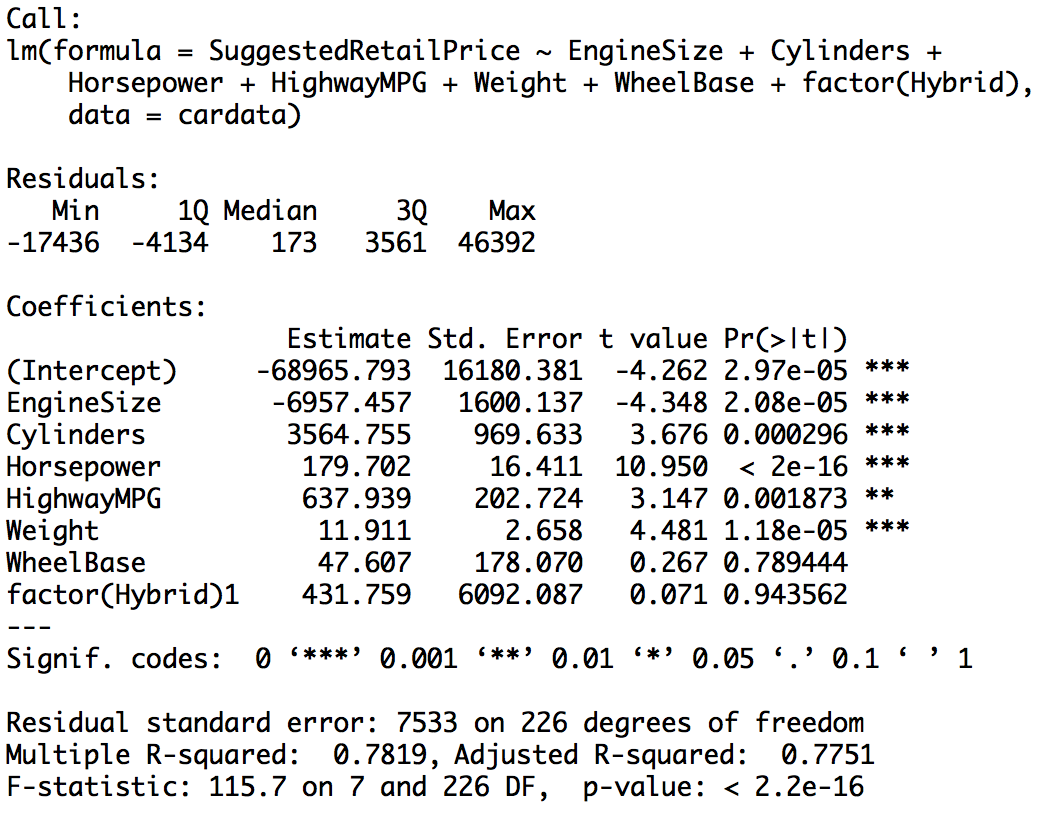
\includegraphics[width=11cm]{Part1_summary_model1}
	\caption{Summary of model 1}
\end{figure}

At first glance it seems that WheelBase and Hybrid aren't important predictors because their p-values are 0.7894 and 0.9436 respectively. This will be confirmed later on in the added variable plots. As we can see in the pairs plot in figure 2, some variables such as HighwayMPG need to be transformed to fit a linear relationship with the response. Figure 3 suggests that the error term isn't constant, since there is a change in the residual's spread over the predicted values. This means that the linear model may not be well suited for the data as it is. From the studentized residuals plot in figure 4, we see that points 222, 229 and 223 are above 4 standard deviations away from the predicted value. However the hat values plot in figure 4 tells us that only point 222 is significantly influent on the response, so we might need to remove it. We'll transform the data first and see if that's still the case.


%  Figure 2: Pairs plot for model 1
\begin{figure}[h!]				
	\centering
	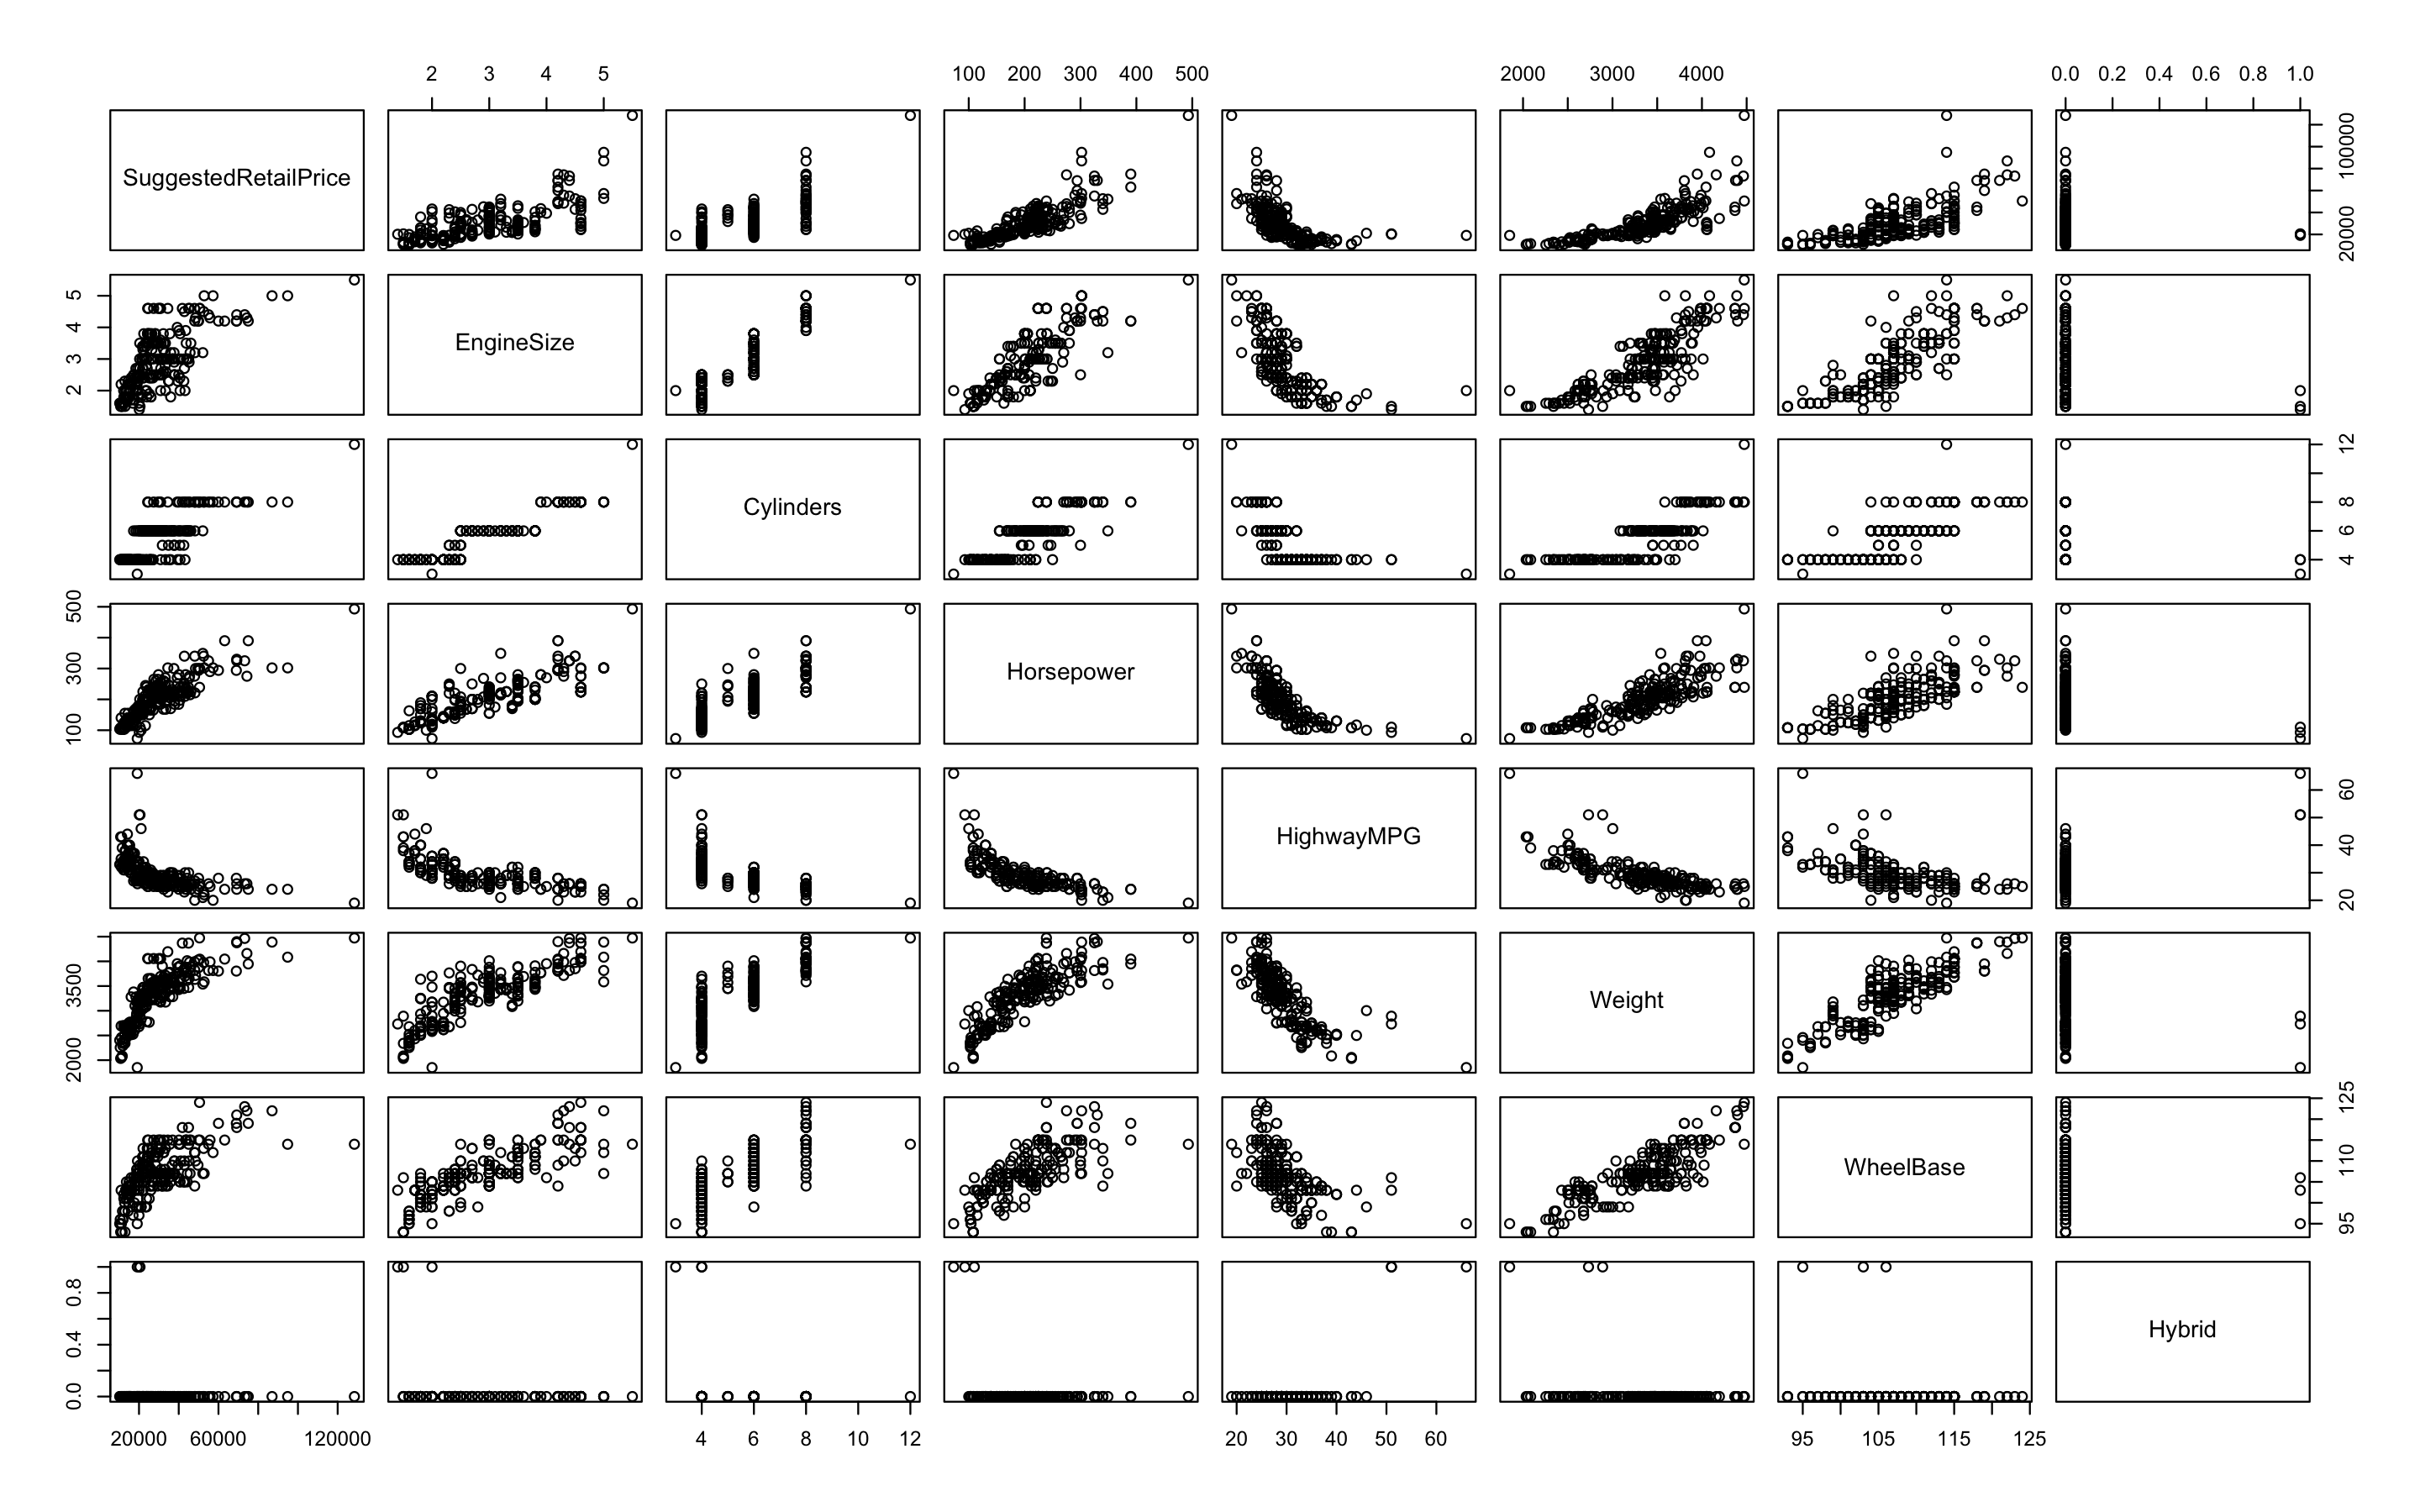
\includegraphics[width=16cm]{Part1_Pairs_Original}
	\caption{Pairs plot for model 1}
\end{figure}

%  Figure 3: residual plot for model 1
\begin{figure}[h!]				
	\centering
	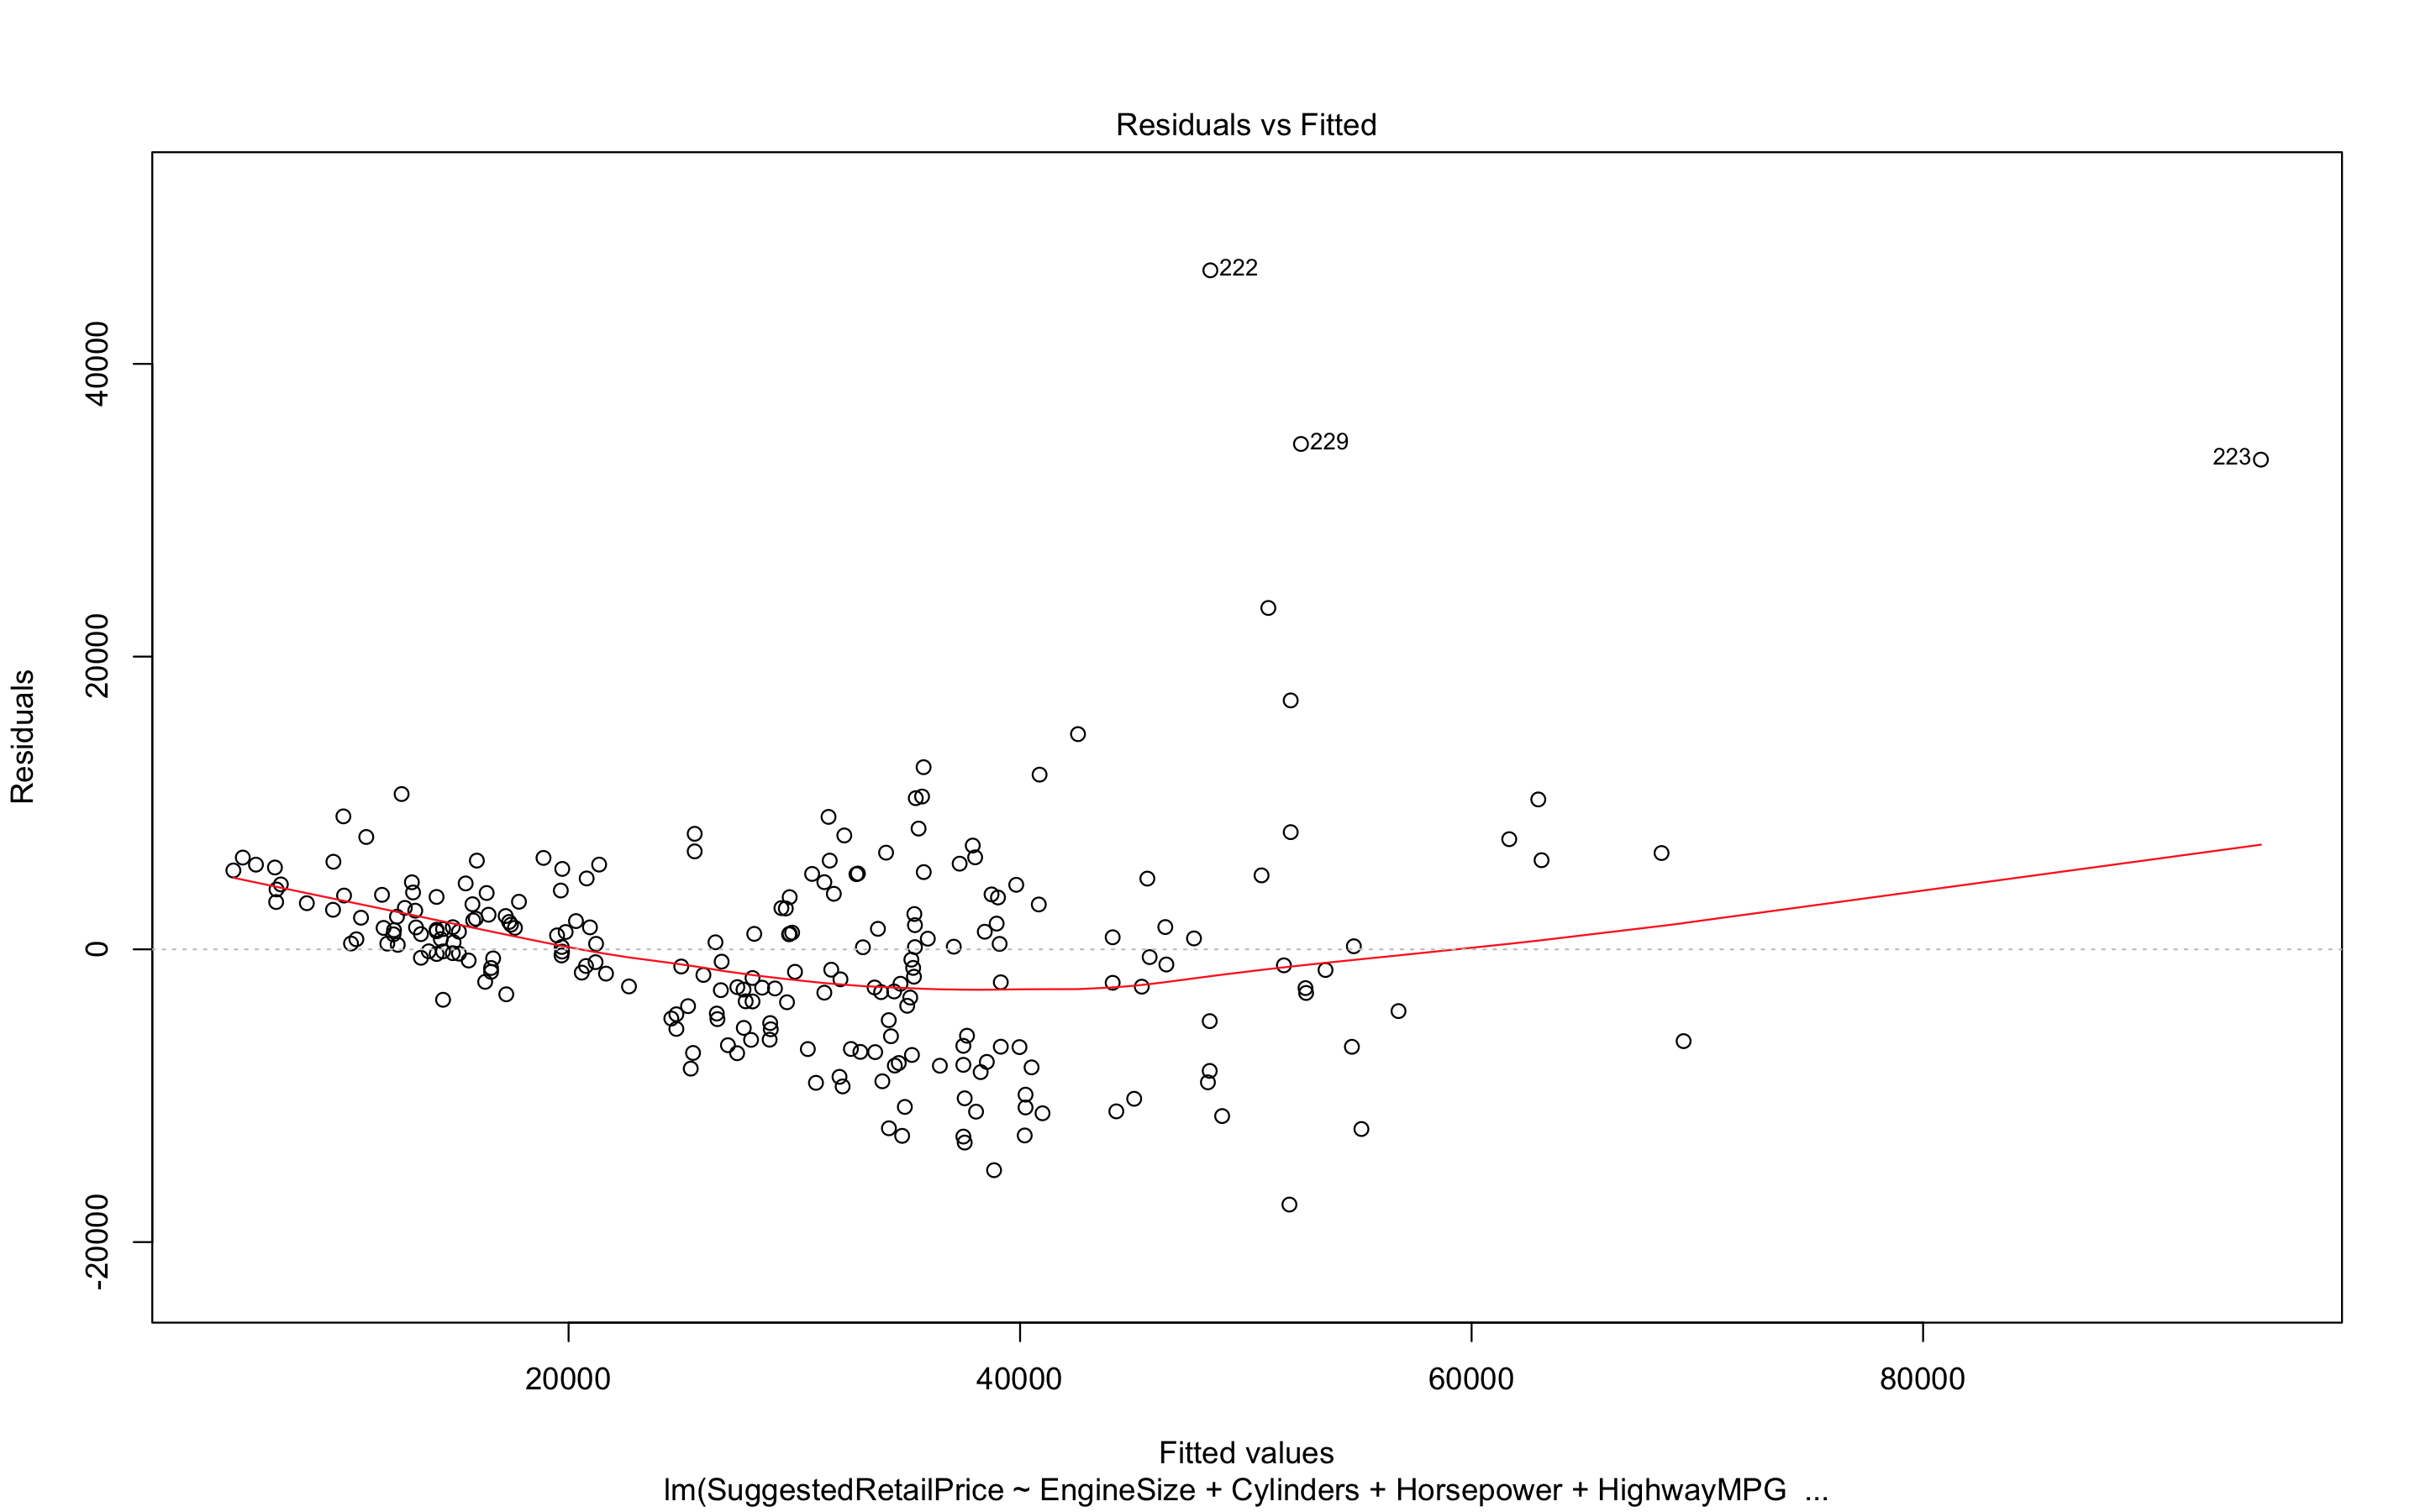
\includegraphics[width=16cm]{Part1_residuals}
	\caption{Residual plot for model 1}
\end{figure}

%  Figure 4: influenceIndex plot for model 1
\begin{figure}[h!]				
	\centering
	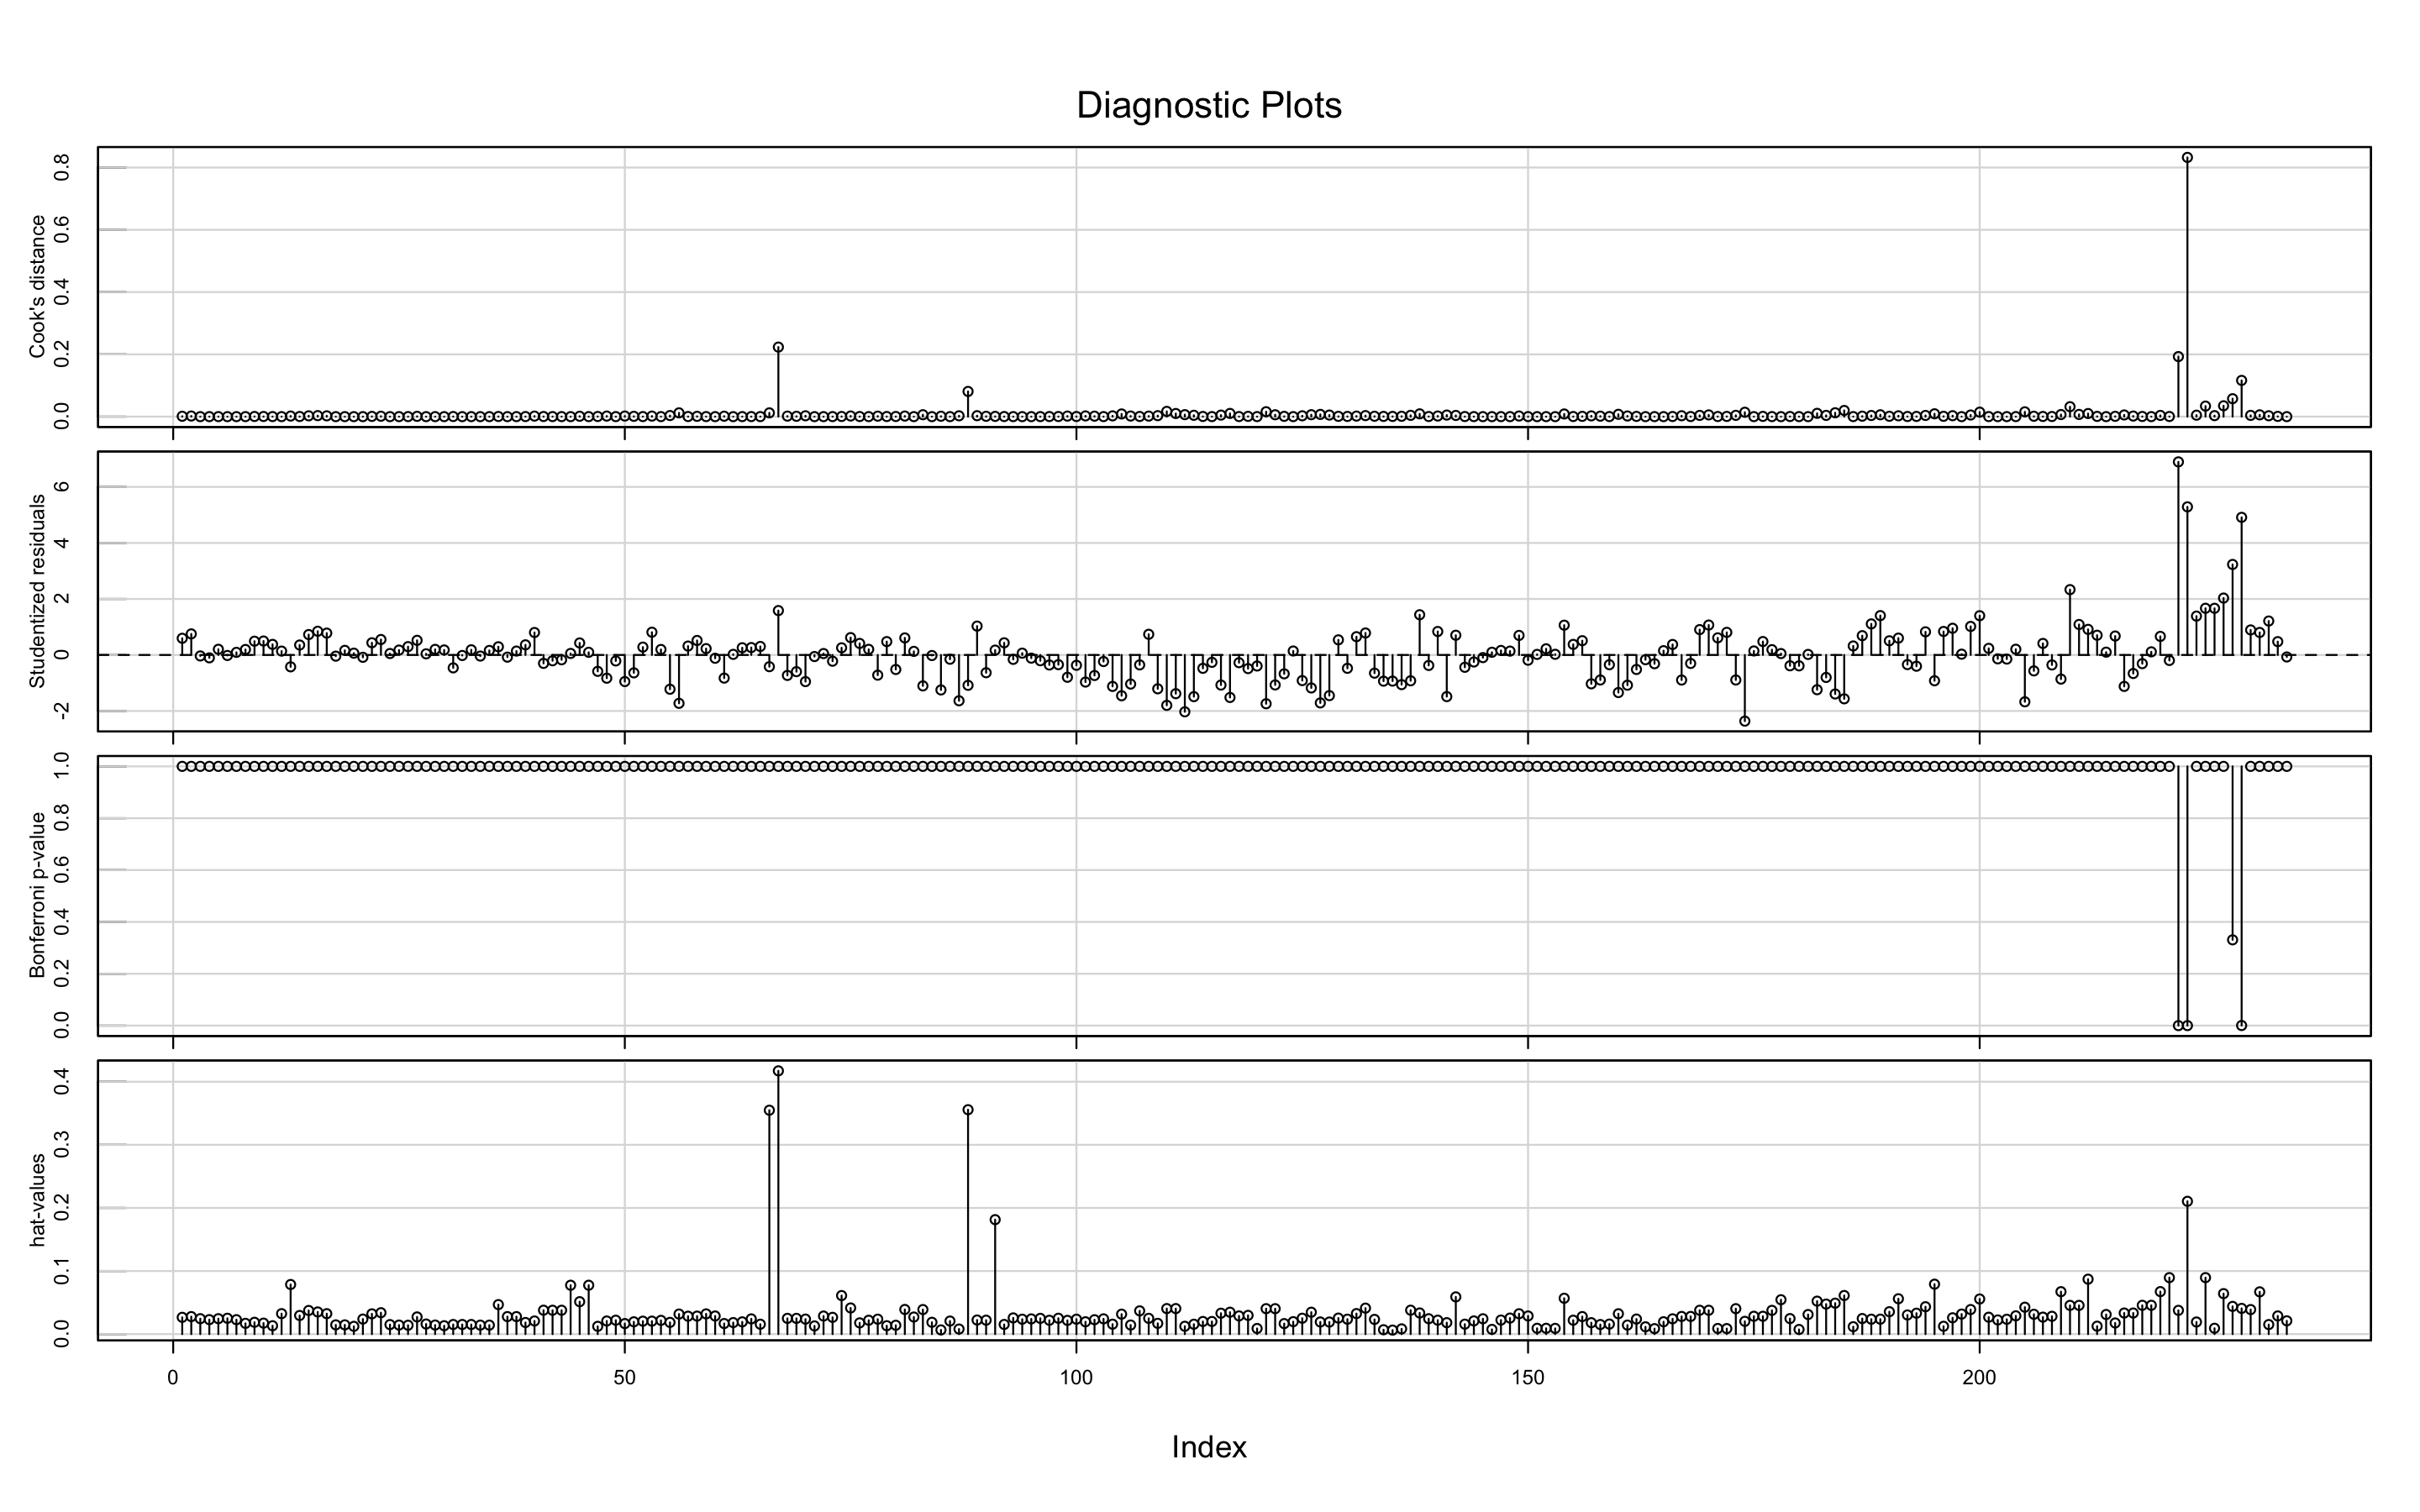
\includegraphics[width=14cm]{Part1_influenceplot}
	\caption{Influence/Index plot for model 1}
\end{figure}

\paragraph{}
The preceding figures strongly suggest that the model could be improved by transforming the variables. A power transformation of the model is performed using the powerTransform function. The transformed variables of model 2 are shown in figure 5. After the power transformation, a new leverage analysis (figure 6) tells us that point 67 is an outlier and is very influential, and point 222 (which hasn't been removed) is no longer an outlier.


%  Figure 5: Pairs plot for model 2
\begin{figure}[h!]				
	\centering
	\includegraphics[width=14cm]{Part1_Pairs_Transformed}
	\caption{Pairs plot for model 2}
\end{figure}

%  Figure 6: influenceIndex plot for model 2
\begin{figure}[h!]				
	\centering
	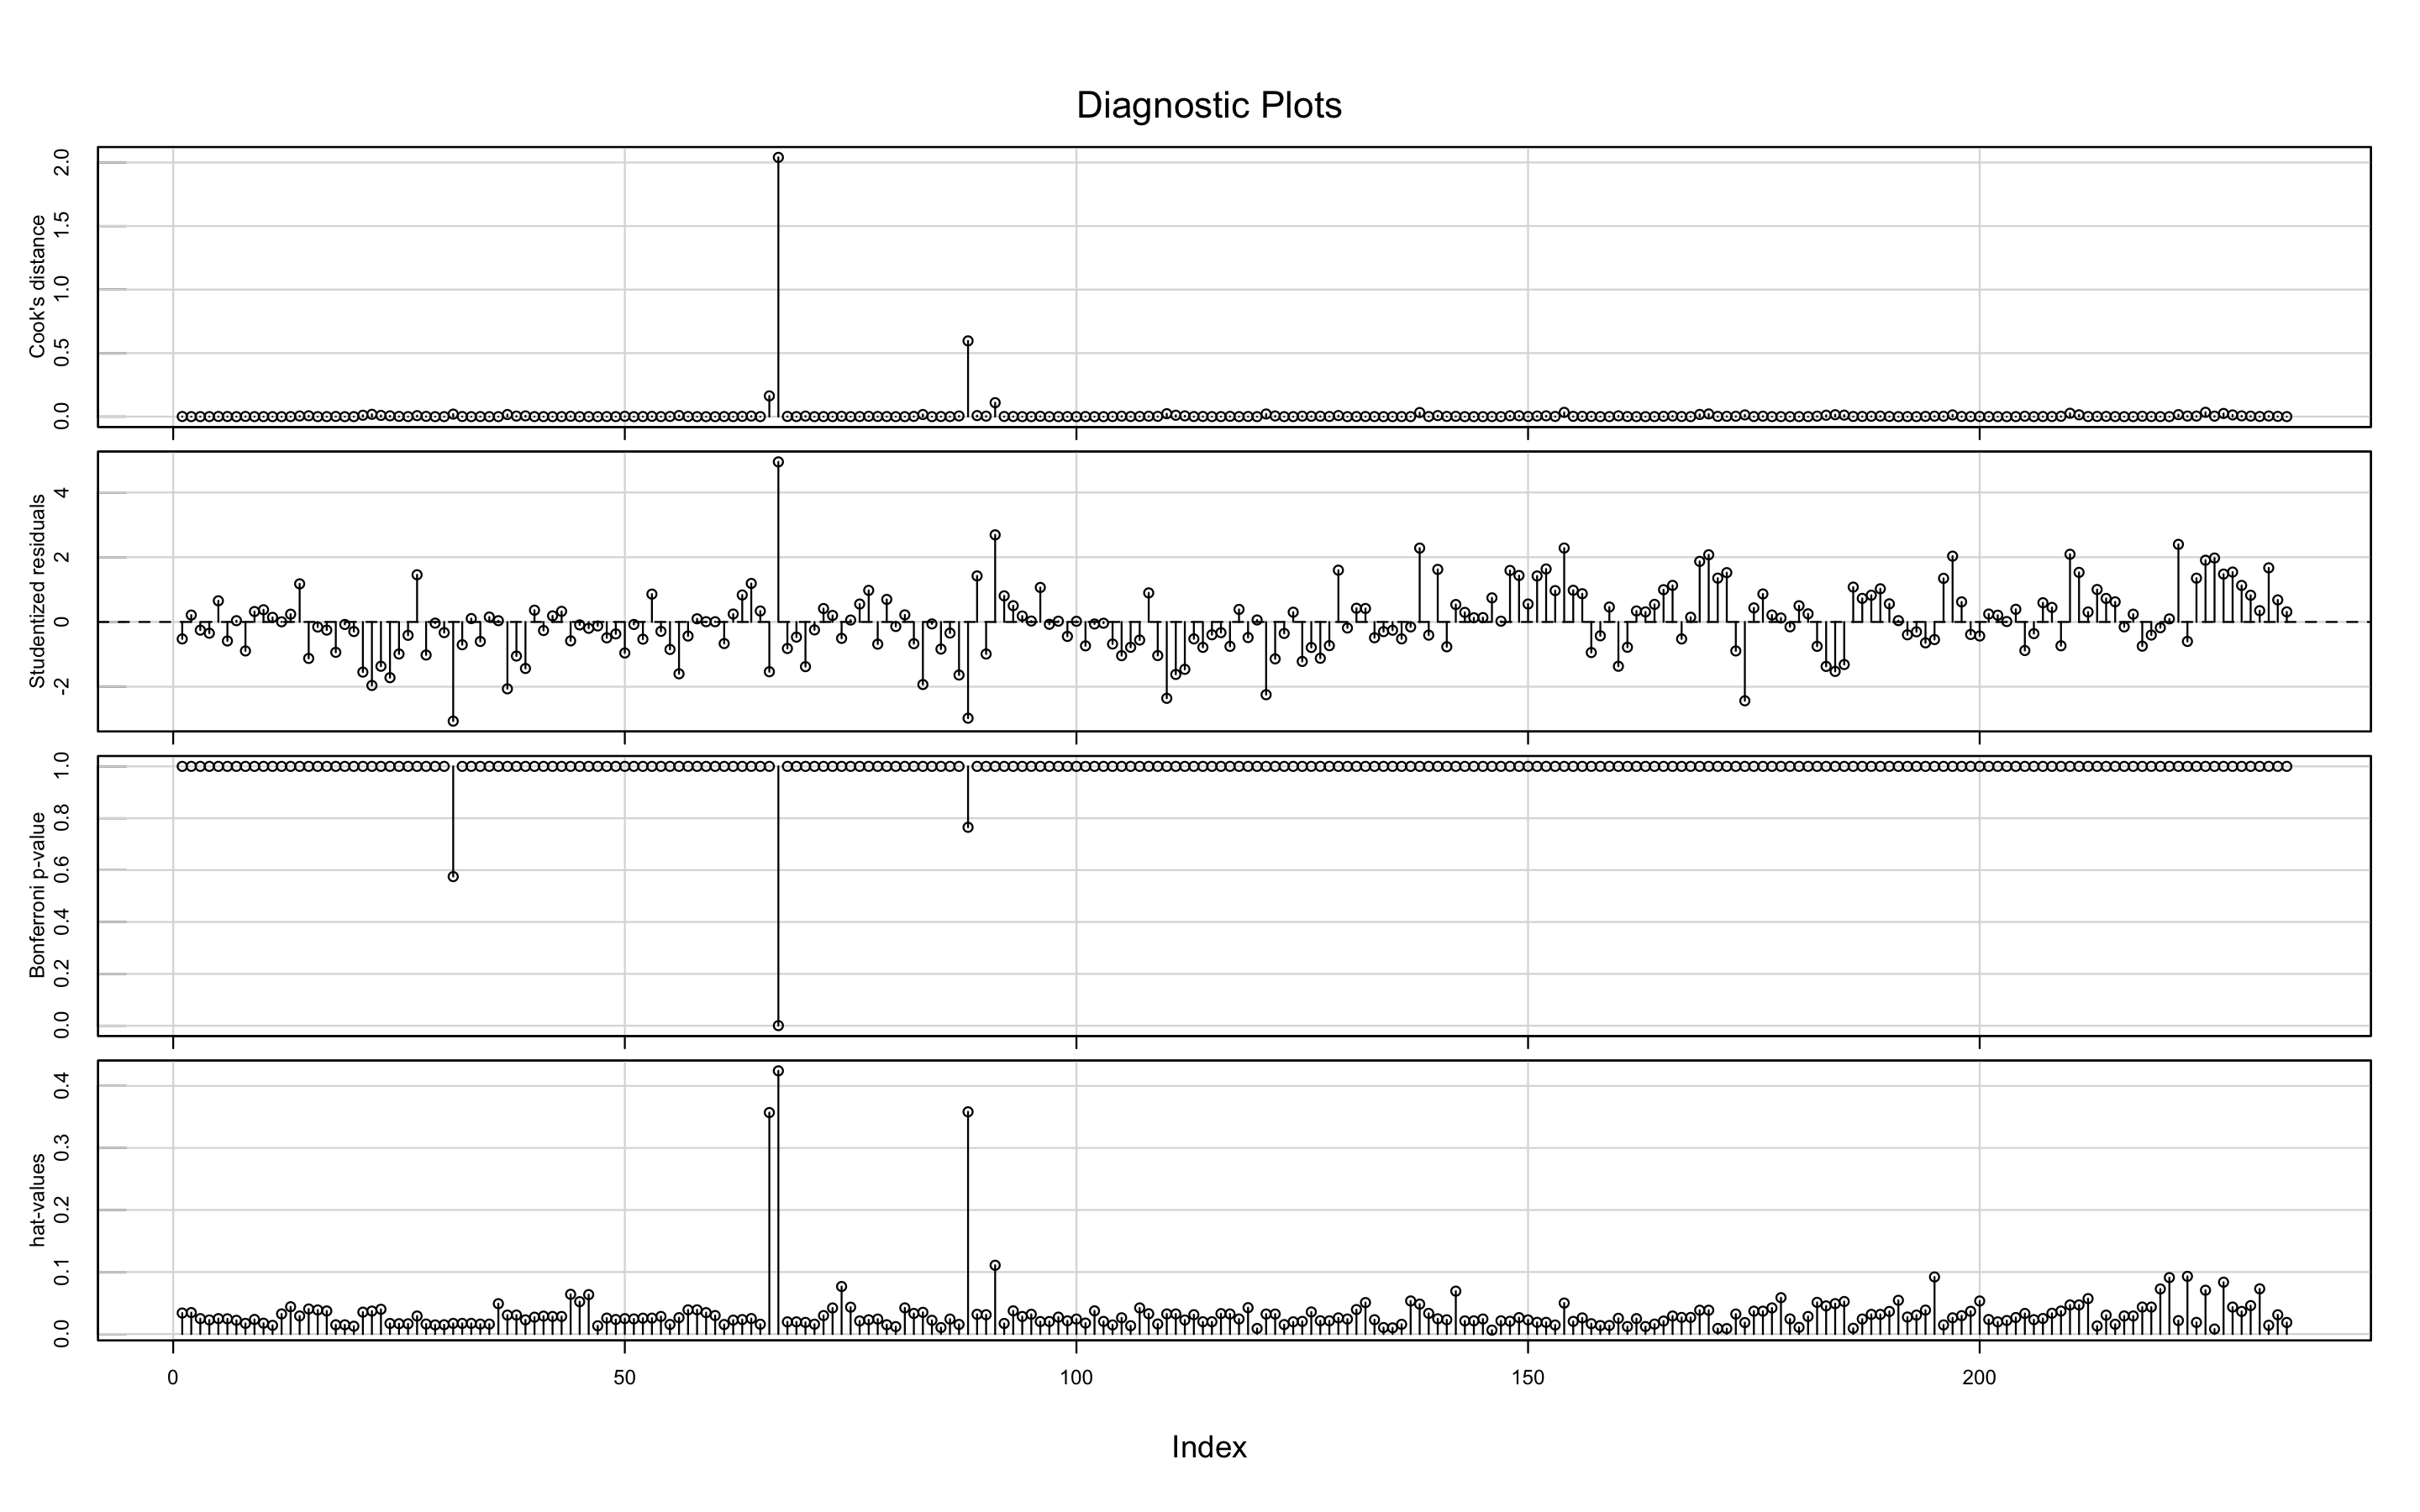
\includegraphics[width=14cm]{Part1_influenceplot_transformed}
	\caption{Influence/Index plot for model 2}
\end{figure}

\paragraph{}
The entry in cardata.txt at index 67 is a hybrid Honda with 3 cylinders, 73 horsepower, 66 highway miles per gallon (all of which are extrema in the dataset) and an engine size of 2.0. This is a very unusual combination of values: with one other exception, all other cars have horsepower values greater than 100, including those with engines of size 1.4. We can therefore assume that this car is a very unlikely occurence, and removing it from the model will not hinder its predictive or descriptive power.

\paragraph{}
After removing the outlier, a new power transformation is carried out (model 3). Weight, EngineSize and Horsepower have the lowest p-values, hence they are the most trustworthy predictors. Their regression coefficients tell us that a unit increase in each of log(EngineSize), log(Horsepower) and Weight causes an increase of -3.61e-03, 5.54e-03 and 3.72e-06 in bcPower(SuggestedRetailPrice, -0.5), respectively. The coefficient of Cylinders, with a p-value of 0.23, has a sizeable chance of being zero, and is already an order of magnitude smaller than the rest of the predictors, which hints that the number of cylinders isn't a good predictor for price. Weight, on the other hand, has a p-value of nearly zero, so the coefficient is very reliable, but still quite low, so not very indicative of a relation with price. Interestingly, the coefficient for EngineSize is negative, which means that it contributes negatively to the price, given all other predictors are fixed.

\paragraph{}
Figure 7 shows the comparison of the summaries of each model. We can see that the p-values of Wheelbase and HighwayMPG in model 3 are very high (0.841 and 0.866 respectively). The added variable plots in figure 8 also give strong evidence that these two variables aren't contributing to the retail price. In the fourth model we remove these two predictors and redo the power transformation. The F-test result for model 3 shown in figure 7 is significantly higher than that of model 2. We can therefore drop the predictors WheelBase and HighwayMPG.

\paragraph{Question 2}
We could introduce a term in the model that accounts for categorical variables using the factor() function. Model 5 introduces such a term, and it was observed that some brands have larger p-values than others, which means that they are more likely to affect the price (given their beta coefficient is high enough in absolute value) than the rest. For example, Chevrolet, Dodge, Chrysler, Ford and Honda cars all have prices in the \$18,000 to \$25,000 range, and similar weights and horsepower (2.7 to 3.5 tons and 150 to 200 Hp respectively). They all have very negative coefficients, and very low p-values. On the other hand, Saab, Volvo and BMW cars have prices roughly in the \$30,000 to \$60,000 range, similar weights and horsepower, and they have positive coefficients and acceptably low p-values. This model is therefore able to relate car brands to prices. We notice however these p-values are higher than those of the cheaper cars. This indicates that the brand correlates with the price much better with cheap cars than with expensive cars, given similar attributes. 


%  Figure 7: Summary of all models
\begin{figure}[h!]				
	\centering
	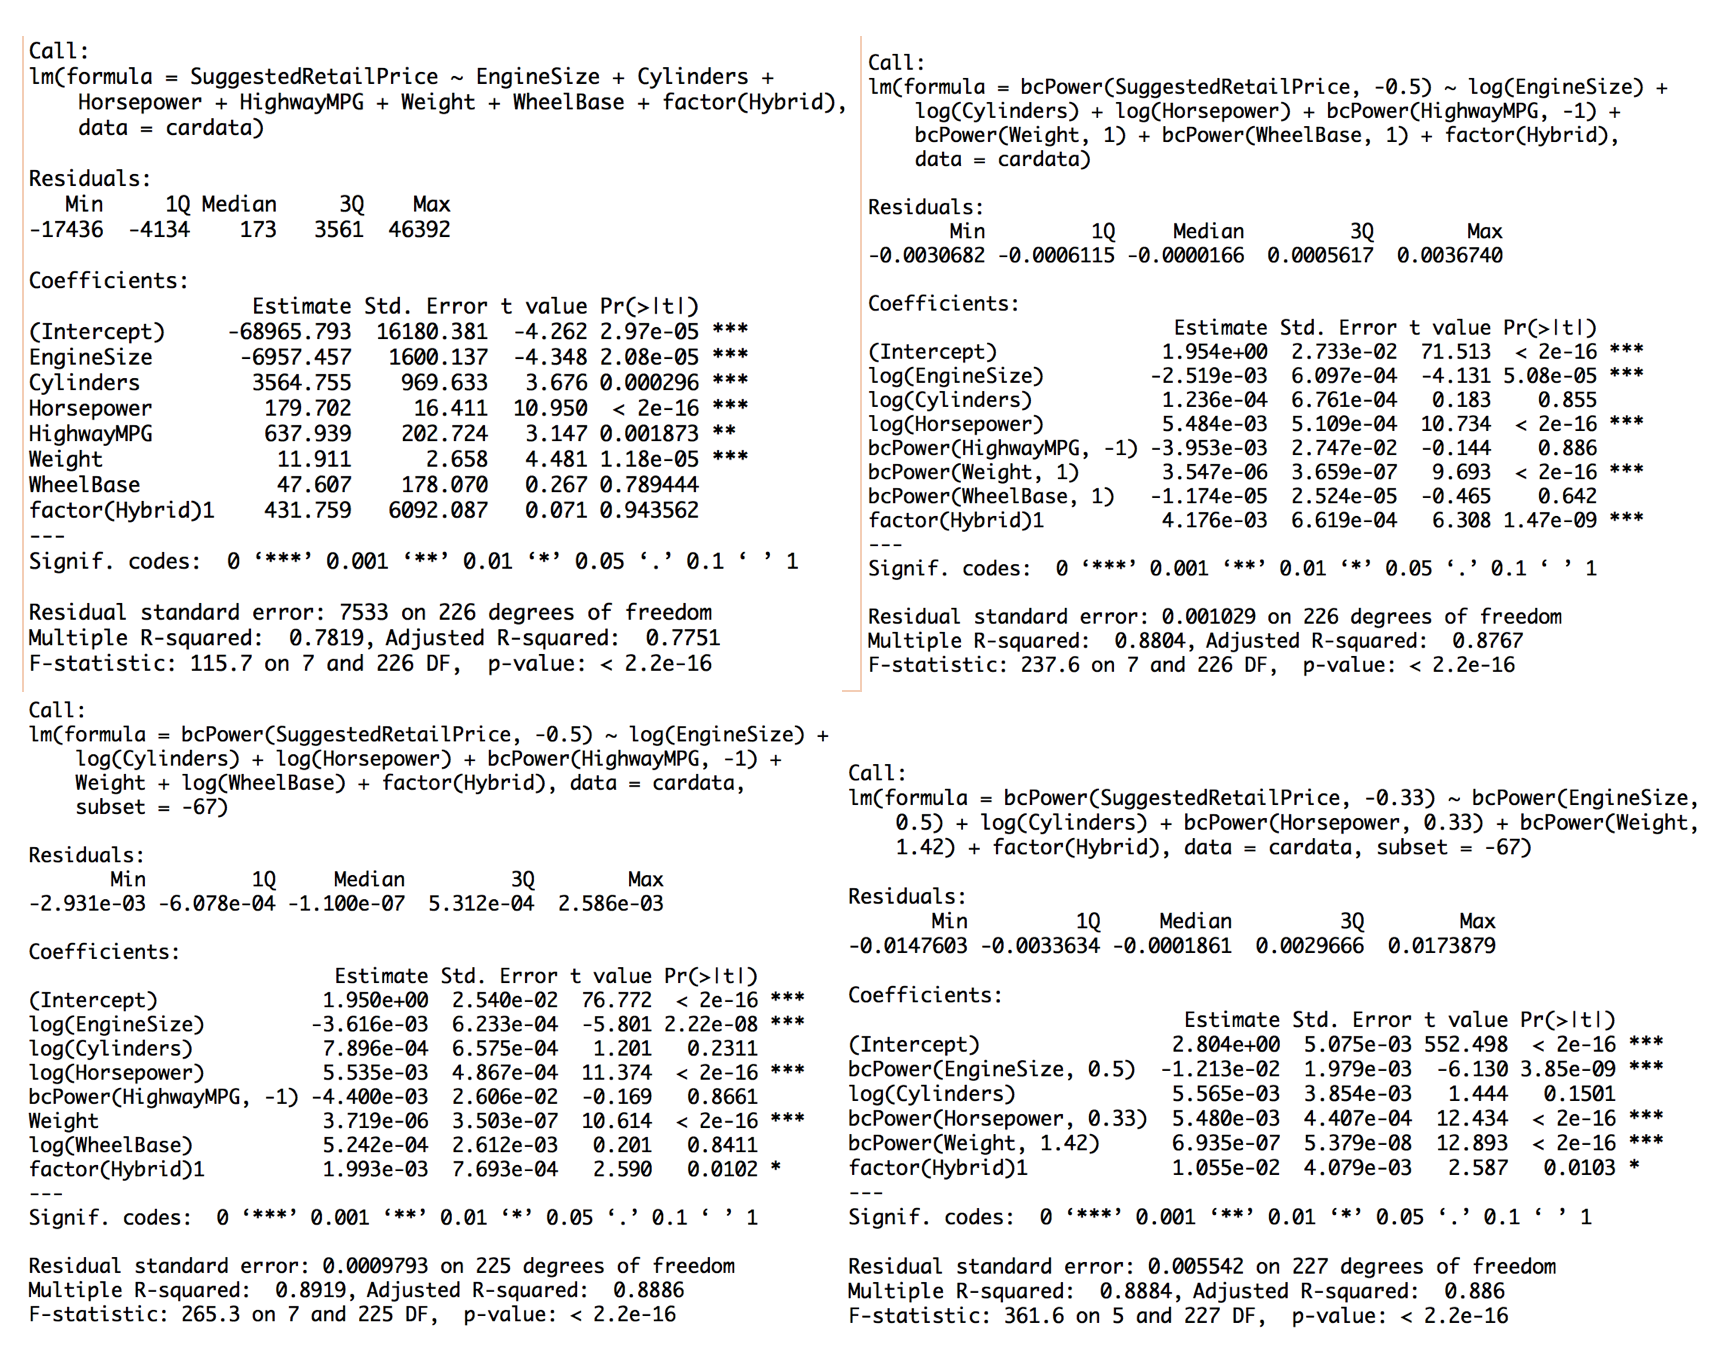
\includegraphics[width=12cm]{Part1_summary_allmodels}
	\caption{Summaries of all models. Clockwise from top left: Model 1, Model 2, Model 4, Model 3}
\end{figure}

%  Figure 8: Added variable plots for model 3
\begin{figure}[h!]				
	\centering
	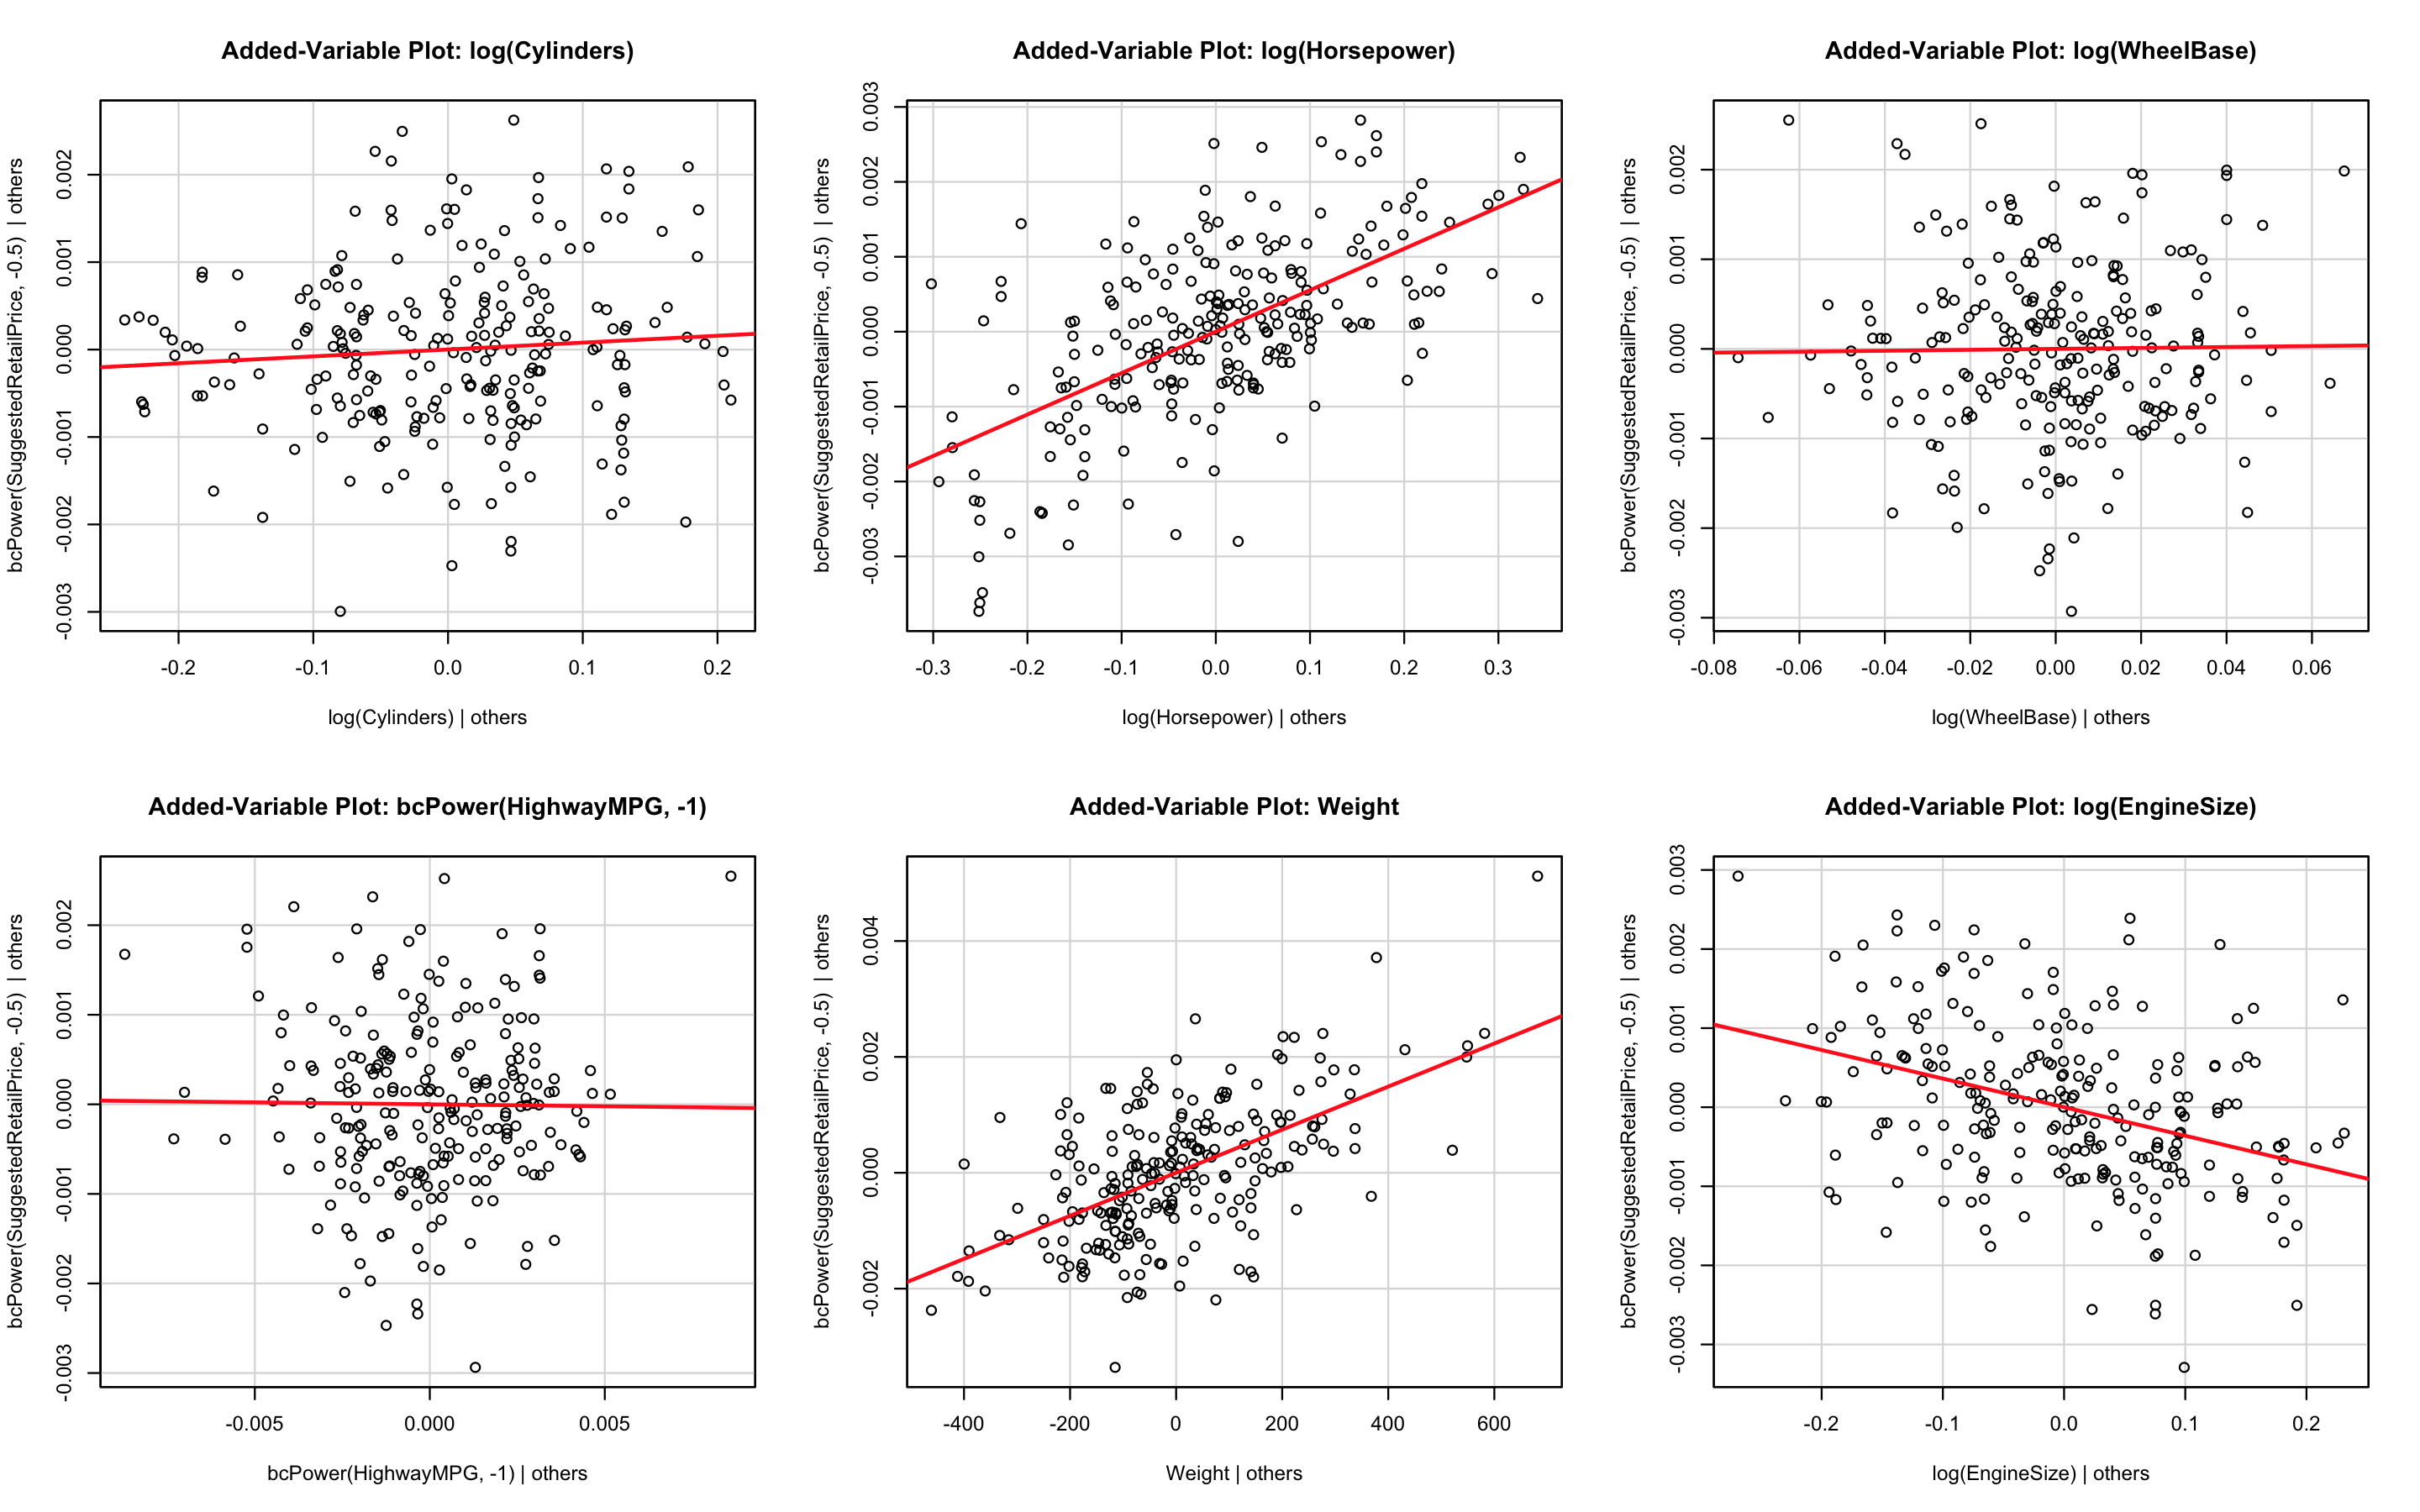
\includegraphics[width=12cm]{Part1_avplots_model3}
	\caption{Added variable plots for model 3}
\end{figure}



\section{Studying the effects of restaurant attributes on dinner prices}

\paragraph{Question 1}
We start by making a linear model of the data. Model 1 contains the variables Price, Food, Decor, Service and East. A pairs plot gives us a general idea of the relationship between the variables.

%  Figure 9: Pairs plot for model 1
\begin{figure}[h!]				
	\centering
	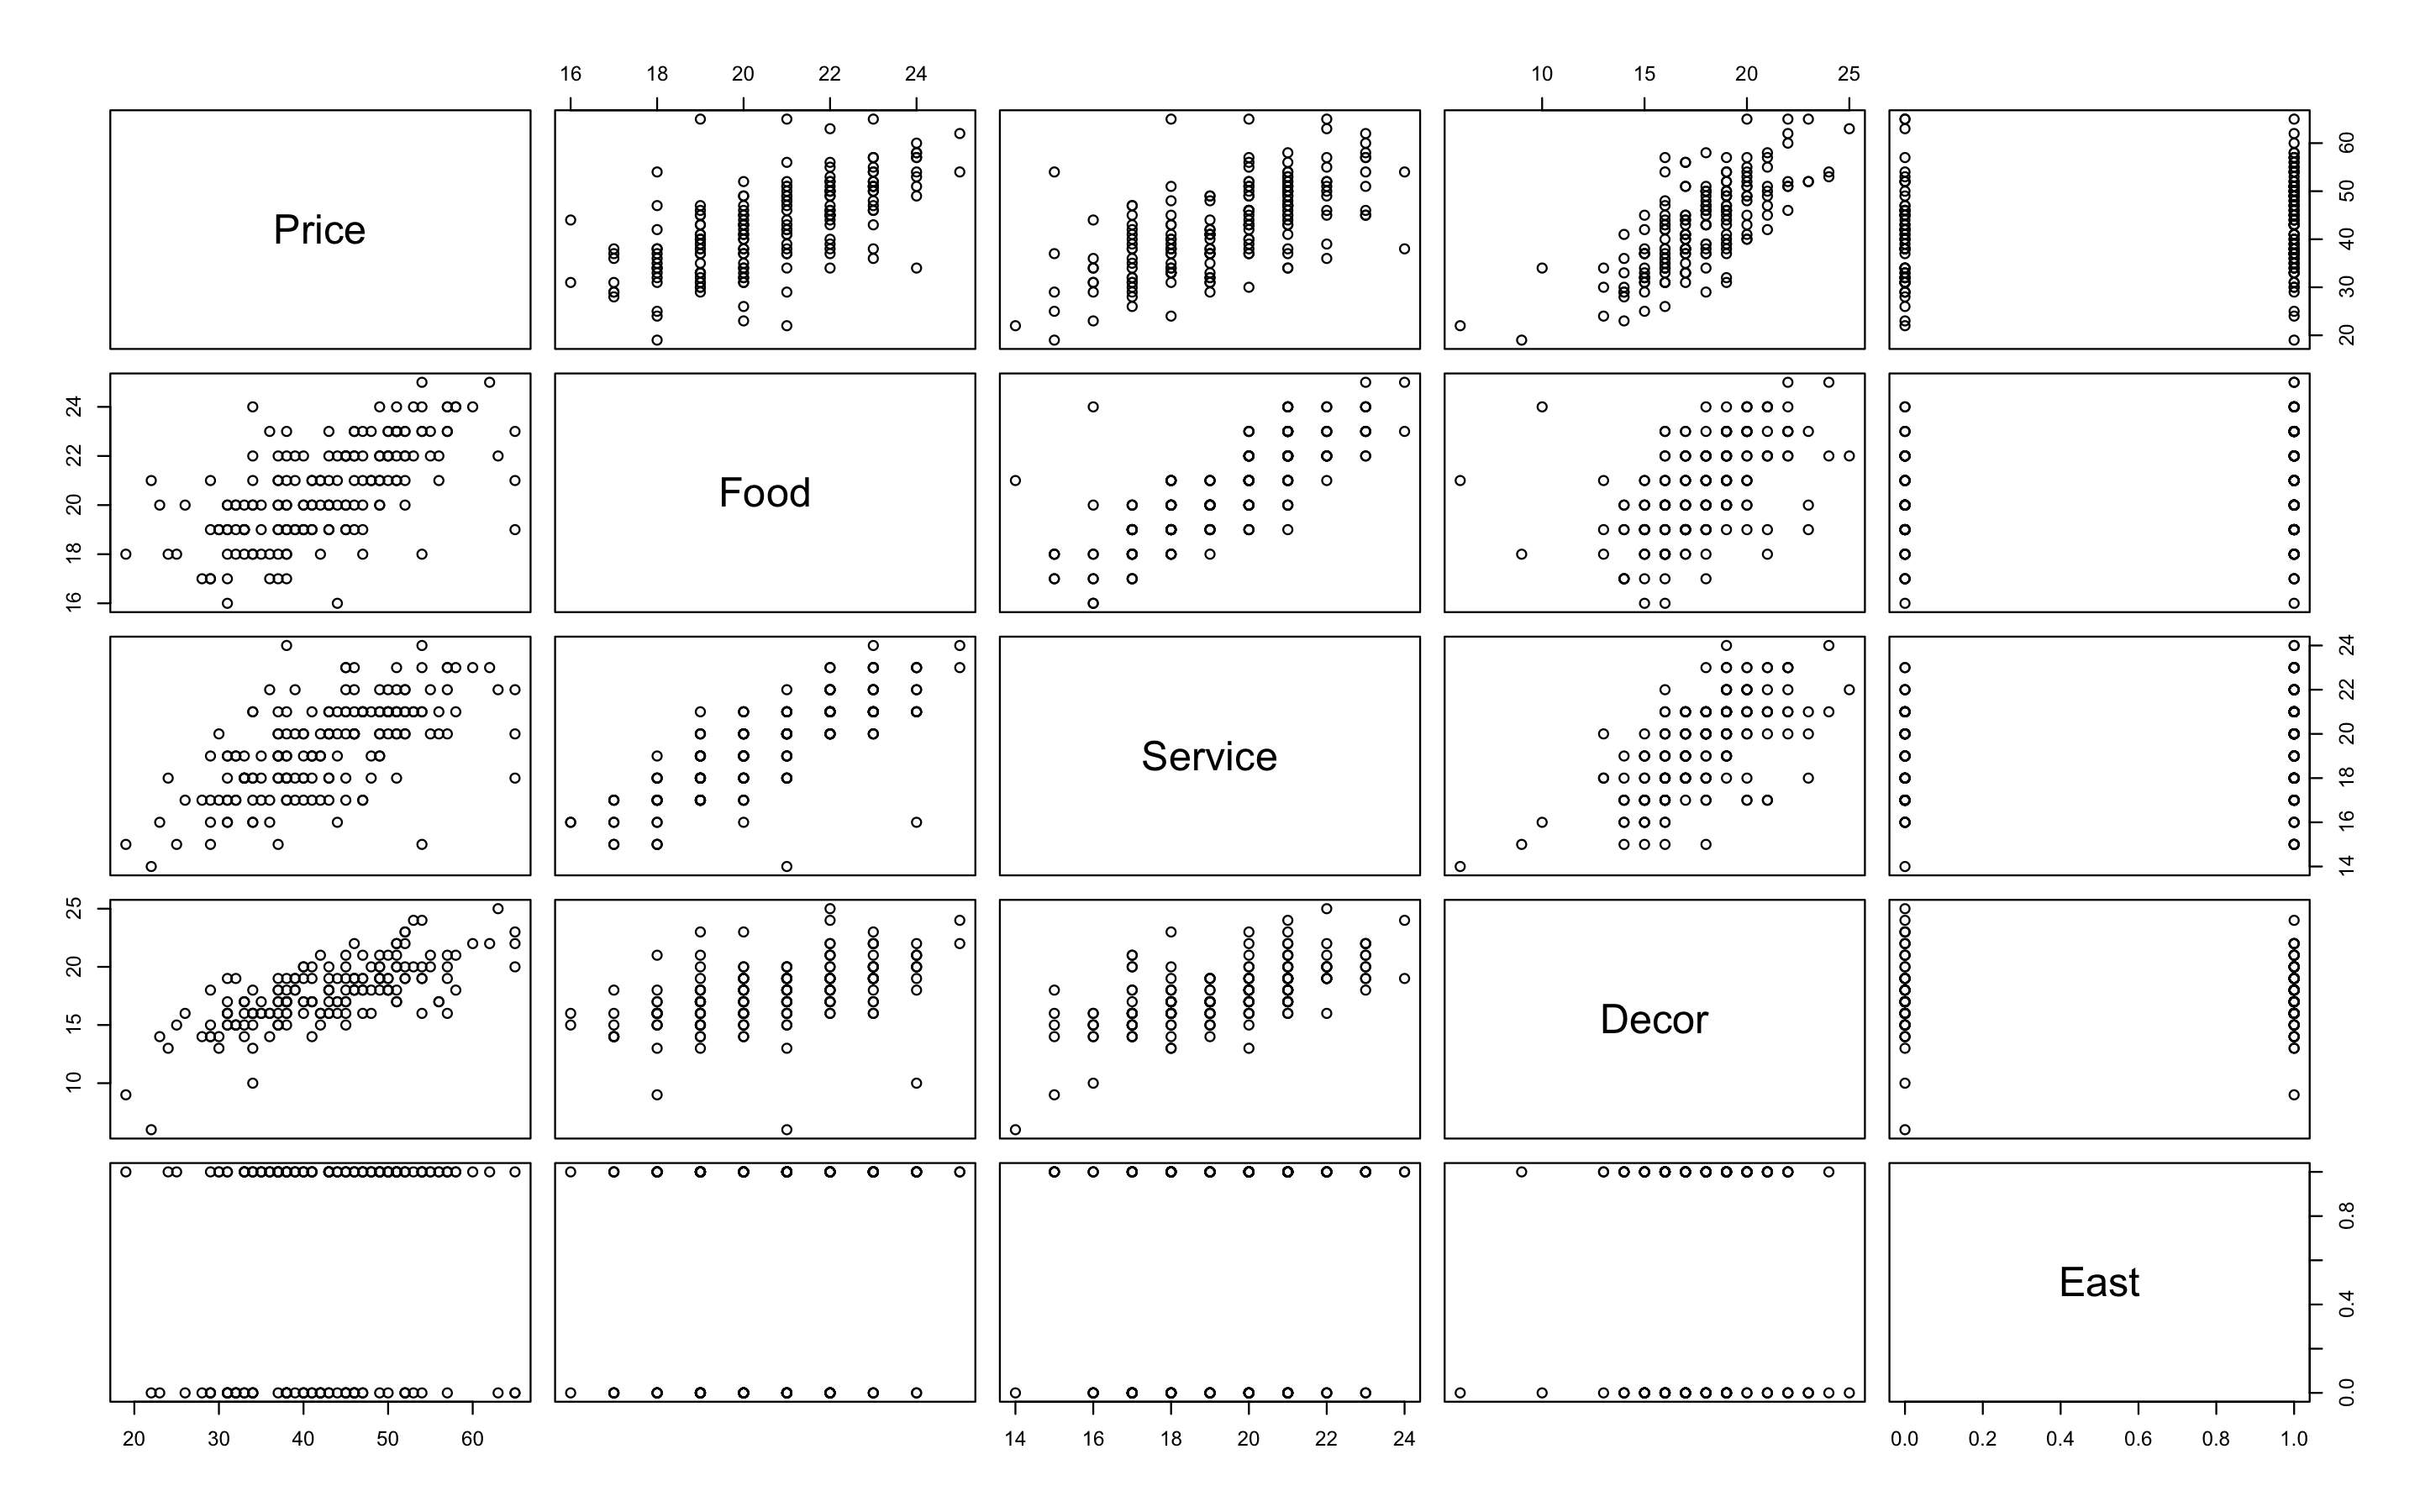
\includegraphics[width=12cm]{Part2_Pairs}
	\caption{Pairs plot for model 1}
\end{figure}

\paragraph{}
It seems that a linear model would fit the data pretty well. A powerTransform() command yields coefficients of 1 for all predictors, which confirms our statement. An influenceIndexPlot() command (figure 10) shows us that points number 56, 30 and 130 are outliers, but they all have very little leverage, so we keep them. 

%  Figure 10: Influence / Index plot for model 1
\begin{figure}[h!]				
	\centering
	\includegraphics[width=13cm]{Part2_influenceplot}
	\caption{Influence / Index plot for model 1}
\end{figure}

\paragraph{}
The summary() command shows us that Service has a very high p-value (0.99) and so can safely be dropped from the model. The coefficients of the resulting model (model 2) are shown in figure 11. Predictably, we see that the restaurant price is highly correlated with the customer ratings for Food and Decor, and a little less so with the location.

%  Figure 11: Summary for model 2
\begin{figure}[h!]				
	\centering
	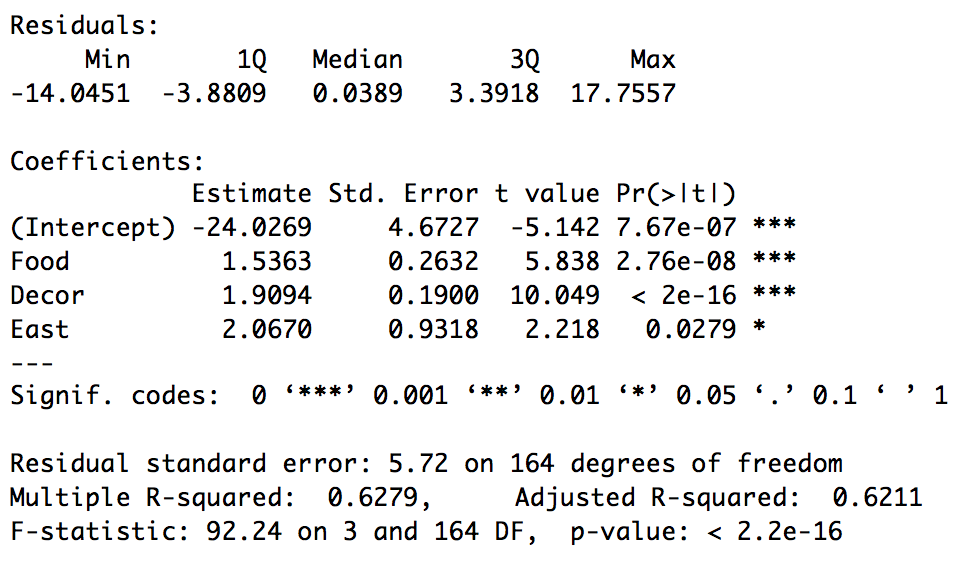
\includegraphics[width=11cm]{Part2_summaryminusservice}
	\caption{Summary for model 2}
\end{figure}

\paragraph{Question 2}
Adding interaction terms Food\_East, Decor\_East and Service\_East, we see that the model doesn't improve much: the F-value decreases from 92 to 40, the new variables have large p-values and their added variable plots are very spread out. Service is still a poor predictor, with a p-value of 0.88 and a beta estimate of -0.05. We can safely say that East doesn't interact much with other predictors, in other words, being on the East side of New York doesn't necessarily increase the effect of the Food, Decor or Service rating on the price. Therefore, there is little evidence for the need to make two separate models for East and West.

%  Figure 12: Summary for model 3
\begin{figure}[h!]				
	\centering
	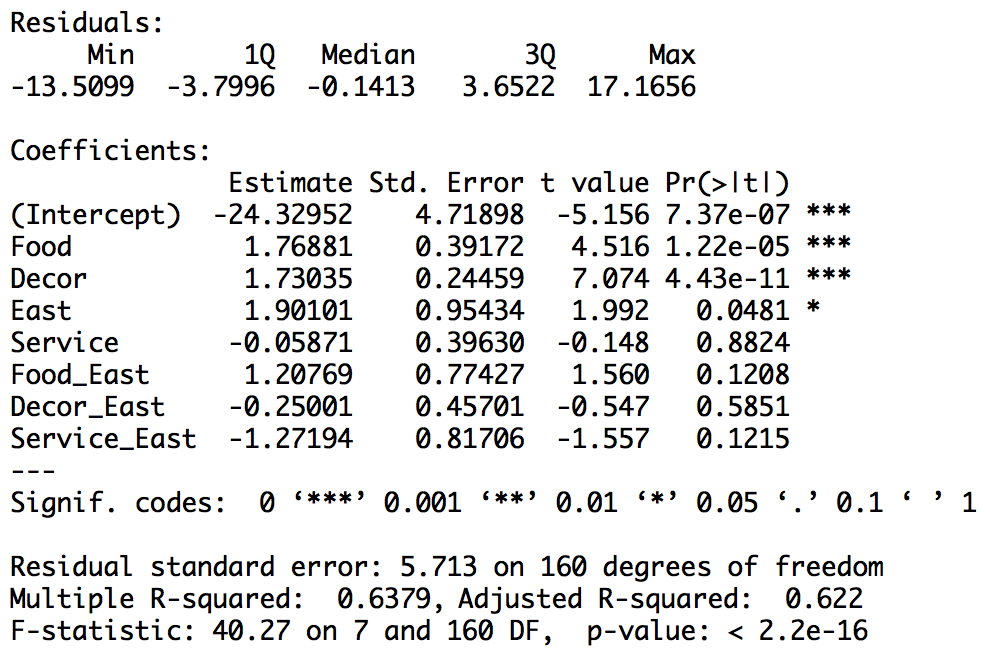
\includegraphics[width=11cm]{Part2_summary_model3}
	\caption{Summary for model 3}
\end{figure}

%  Figure 13: Added variable plots for model 3
\begin{figure}[h!]				
	\centering
	\includegraphics[width=16cm]{Part2_avplots_interaction}
	\caption{Added variable plots for model 3}
\end{figure}


\end	{document}